\input{head.inc}

% Präambelbefehle für die Präsentation
\title[TET: Stationäres Elektrisches Strömungsfeld]{Stationäres Elektrisches Strömungsfeld}

\begin{document}
% 
% Frontmatter 
% 
%%%%%%%%%%%%%%%%%%%%%%%%%%%%%%%%%%%%%%%%%%%%%%%%%%%%%%%%%%%%%%%%%%%%%%%%%%%%%%%%%%%%%%%%%%%%%%%%%%%%%%%%%%%%%%%%%%%%%%%%%%%%% 

%% inserts the title page and the table of contents
\maketitle

% 
% Content 
% 
%%%%%%%%%%%%%%%%%%%%%%%%%%%%%%%%%%%%%%%%%%%%%%%%%%%%%%%%%%%%%%%%%%%%%%%%%%%%%%%%%%%%%%%%%%%%%%%%%%%%%%%%%%%%%%%%%%%%%%%%%%%%% 
\section{Stationäres Elektrisches Strömungsfeld}

\begin{frame}

  \frametitle{Ausgangspunkt Elektrostatik}

  \begin{itemize}[<+->]
    \item Maxwell-Gleichungen:
\begin{align*}
	& \rotation\EFeld[v] = \underbrace{-\dfrac{\partial \BFeld[v]}{\partial t}}_{=\vec{0}} = \vec{0} \\
	& \divergenz \DFeld[v] = \laddichte{V} 
\end{align*}
\item Elektrostatik $\to$ \alert{ruhenden} Ladungen $\to$ \alert{elektrostatisches Feld}
\item Jetzt: \alert{Bewegung von Ladungen zugelassen}
  \item Allerdings Beschränkung auf \alert{stationäre Bewegung}:
\begin{equation*}
	\dfrac{\partial}{\partial t} \laddichte{V} = 0 
      \end{equation*}
 \item Es existiert somit eine Stromdichte \alert{\(\StromDichte[v] \neq \vec{0} \)}.
\end{itemize}

\end{frame}

\begin{frame}
  \frametitle{Stromdichte}


\begin{itemize}[<+->]
    \item Grundsätzlich sind zwei Arten der Bewegung von Ladungsträgern zu betrachten:
  \begin{itemize}[<+->]
    \item Thermische Bewegung \({\Geschwindigkeit[v]}_\mathrm{th}\): Trägt makroskopisch nicht zur Stromdichte \(\StromDichte[v]\) bei, da \(\mittelwert{\Geschwindigkeit[v]_\mathrm{th}} = \vec{0} \).
    \item Driftbewegung \({\Geschwindigkeit[v]}_\mathrm{D}\): Trägt zur Stromdichte \(\StromDichte[v] \) bei, da für den Mittelwert der Driftgeschwindigkeit \(\mittelwert{\Geschwindigkeit[v]_\mathrm{D}} \ne \vec{0} \) gilt.
\end{itemize}
\item Die Driftbewegung muss von einer Kraft getrieben werden.
\item aus dem elektrischen Feld: \(\kraft[v]_\mathrm{\EFeld} = \partladung \cdot \EFeld[v] \)
\item aus dem magnetischen Feld: \(\kraft[v]_\mathrm{\HFeld} = \partladung \cdot \left(\Geschwindigkeit[v] \times \BFeld[v]\right) \) $\to$ in der Regel sehr klein 
\end{itemize}
\end{frame}

\begin{frame}
  \frametitle{Strom}

 \begin{columns}
   \begin{column}{.3\linewidth}
\resizebox{\columnwidth}{!}{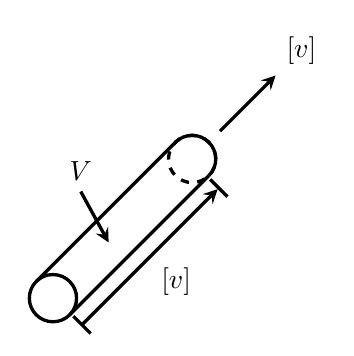
\begin{tikzpicture}[line width = 1.2pt, line join=round,x={(-0.35355cm,-0.35355cm)},y={(1cm, 0cm)},z={(0cm,1cm)},>=stealth]
	% Querschnittsflächen
	\draw [dashed] (0,0) circle (0.3cm);
	\draw (0,0,0)++(0,{0.3*sqrt(2)/2},{-0.3*sqrt(2)/2}) arc (-45:135:0.3cm);
	\draw (5,0) circle (0.3cm);
	% Begrenzungen
	\coordinate (a) at (5,0,0);
	\coordinate (ah) at (2.5,{0.5*sqrt(2)/2},{-0.5*sqrt(2)/2});
	\draw (0,{0.3*sqrt(2)/2},{-0.3*sqrt(2)/2}) -- ++(a);
	\draw (0,{-0.3*sqrt(2)/2},{0.3*sqrt(2)/2}) -- ++(a);
	% differentielles Wegstück
	\draw [|<-|] (0,{0.5*sqrt(2)/2},{-0.5*sqrt(2)/2}) -- ++(a);
	\draw (ah) node[anchor=north west] {$\upd \weg[v]$};
	% Geschwindigkeit
	\draw [->] (-1,0,0) -- (-3,0,0) node[anchor=south west] {$\geschw[v]$};
	% ladungsdichte
	\draw [<-] (3,0,0) -- (4,0,1) node[anchor=south] {$\laddichte{V}$};
\end{tikzpicture}}

\resizebox{\columnwidth}{!}{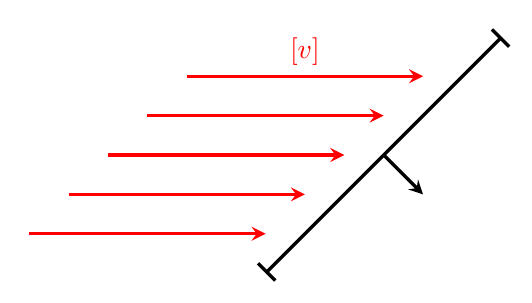
\begin{tikzpicture}[line width = 1.2pt, line join=round,x=1cm,y=1cm,>=stealth]
	% Fläche
	\draw [|-|] (0,-0.5) -- (3,2.5);
	\draw (2.8,2.5) node[anchor=east] {$\spezflaeche$};
	\draw[->] (1.5,1) -- (2,0.5) node[anchor=north west] {$\normalenvektor$};
	% elektrische Stromdichte
	\foreach \s in {0,0.5,1,1.5,2} \draw[->,color=red] ({-3+\s},{\s}) -- ({\s},{\s});
	\draw [color=red] (0.5,2) node[anchor=south] {$\elstromdichte[v]$};
\end{tikzpicture}}
   \end{column}
   \begin{column}{.7\linewidth}
\begin{itemize}[<+->]
    \item Für einen Leiter gilt
\begin{equation*}
	\StromDichte[v] = \laddichte{V} \cdot \Geschwindigkeit[v] \pointspacek
\end{equation*}
mit
\begin{align*}
	& \left[\laddichte{V} \right] = \si{\ampere\second\per\cubic\metre} \pointspacek
		&& \left[\Geschwindigkeit \right] = \si{\metre\per\second}\pointspacek
		&& \left[\StromDichte[v] \right] = \si{\ampere\per\square\metre}
\end{align*}
\item Der Gesamtstrom durch die Fläche \(\SpezialFlaeche[v] \) berechnet sich nach
\begin{align*}
	\Strom &= \iint\limits_{\SpezialFlaeche} \StromDichte[v] \cdot \intnach{\SpezialFlaeche[v]} 
		= \iint\limits_{\SpezialFlaeche} \StromDichte[v] \cdot \normalenvektor \intnach{\SpezialFlaeche}
			= \iint\limits_{\SpezialFlaeche} \StromDichte\normal \intnach{\SpezialFlaeche}
\end{align*}
mit
\begin{equation*}
	\StromDichte\normal = \StromDichte[v] \cdot \normalenvektor \pointspacep
\end{equation*}

\end{itemize}
     \end{column}
\end{columns}  
\end{frame}


\begin{frame}
  \frametitle{Ladungserhaltung - Kontinuitätsgleichung}
	\centering
	\resizebox{.25\linewidth}{!}{\begin{tikzpicture}[line width = 1.2pt, line join=round,x=1cm,y=1cm,>=stealth]
	% Koordinaten des Volumens
	\coordinate (a) at (3,0);
	\coordinate (b) at (3.5,0.5);
	\coordinate (c) at (3.1,0.8);
	\coordinate (d) at (3.2,1.2);
	\coordinate (e) at (2.9,1.6);
	\coordinate (f) at (3.0,2.1);
	\coordinate (g) at (2.3,2.2);
	\coordinate (h) at (2,2.4);
	\coordinate (i) at (1.3,1.7);
	\coordinate (j) at (0,2.3);
	\coordinate (k) at (-0.9,1.9);
	\coordinate (l) at (-1.7,2.3);
	\coordinate (m) at (-2.6,1.9);
	\coordinate (n) at (-2.5,1.6);
	\coordinate (o) at (-2.8,1.4);
	\coordinate (p) at (-3,0.8);
	\coordinate (q) at (-2.1,-0.1);
	\coordinate (r) at (-2.8,-0.9);
	\coordinate (s) at (-2.6,-1.8);
	\coordinate (t) at (-1.9,-2.1);
	\coordinate (u) at (-1.2,-2.9);
	\coordinate (v) at (-0.6,-2.3);
	\coordinate (w) at (0.1,-2.5);
	\coordinate (x) at (0.9,-1.9);
	\coordinate (y) at (1.6,-2.2);
	\coordinate (z) at (2.7,-1.2);
	% Volumen
	\draw [color=darkgreen] plot [smooth cycle, tension=0.8] coordinates {(a) (b) (c) (d) (e) (f) (g) (h) (i) (j) (k) (l) (m) (o) (p) (q) (r) (s) (t) (u) (v) (w) (x) (y) (z)};
	\shade [ball color=white!20!darkgreen, opacity=0.20] plot [smooth cycle, tension=0.8] coordinates {(a) (b) (c) (d) (e) (f) (g) (h) (i) (j) (k) (l) (m) (o) (p) (q) (r) (s) (t) (u) (v) (w) (x) (y) (z)};
	\draw [color=darkgreen] plot [smooth, tension=0.8] coordinates {(a) (2.6,-0.6) (2,-0.3) (0.7,-1) (-1,-0.4) (-1.7,-0.3) (q)};
	\draw [color=darkgreen, dashed] plot [smooth, tension=0.8] coordinates {(a) (2.7,0.4) (1.9,0.3) (0.9,0.7) (-1.6,0.4) (q)};
	\draw [color=darkgreen!80!black] (-2,1) node {$ \volumen $};
	\draw [color=darkgreen!80!black] (-2,-1) node {$ \laddichte{V} $};
	% Normalenvektoren
	\draw [->] (q) -- ++(-0.9,-0.05) node[anchor=east] {$ \normalenvektor $};
	\draw [->] (h) -- ++(-0.14,0.8) node [anchor=south] {$ \normalenvektor $};
	\draw [->] (b) -- ++(0.9,-0.05) node[anchor=west] {$ \normalenvektor $};
	\draw [->] (y) -- ++(0.35,-0.6) node[anchor=north] {$ \normalenvektor $};
	\draw [->] (t) -- ++(-0.6,-0.5) node[anchor=north east] {$ \normalenvektor $};
	\draw [->] (l) -- ++(0.05,0.6) node[anchor=south east] {$ \normalenvektor $};
	\draw [->] (-0.3,0) -- ++(-0.2,0.3) node[anchor=south] {$ \normalenvektor $};
	% Stromdichten
	\draw [color=red] (-3.7,1) node {$ \StromDichte[v] $};
	\draw [color=red] (4,1.6) node {$ \StromDichte[v] $};
		% hineinflie�end
		\draw [<-,color=red] (m) -- ++(-0.4,0.5);
		\draw [<-,color=red] (s) -- ++(-0.4,-0.3);
		\draw [<-,color=red] (o) -- ++(-0.8,0.1);
		\draw [<-,color=red] (r) -- ++(-0.6,0.3);
		\draw [<-,color=red] (k) -- ++(0.1,0.8);
		\draw [<-,color=red] (u) -- ++(-0.1,-0.7);
		\draw [->,color=red] (-1.7,-1.5) -- ++(0.2,0.1);
		% herausflie�end
		\draw [->,color=red] (z) -- ++ (0.5,-0.4);
		\draw [->,color=red] (g) -- ++ (0.4,0.5);
		\draw [->,color=red] (d) -- ++ (0.8,0.1);
		\draw [->,color=red] (a) -- ++ (0.7,-0.2);
		\draw [->,color=red] (w) -- ++ (0.1,-0.8);
		\draw [->,color=red] (i) -- ++ (-0.05,0.5);
		\draw [->,color=red] (2.1,0.8) -- ++(0.2,0.1);
\end{tikzpicture}}
\begin{itemize}[<+->]
    \item Axiomatische Grundlagen: \alert{Ladungserhaltung}
\item Nettostrom durch eine geschlossene Oberfläche $\ne$ Null $\to$ Ladungsdichte des Volumens zeitabhängig
\begin{equation*}
	\dfrac{\partial \laddichte{V}}{\partial t} \neq 0 \pointspacep
\end{equation*}
\item Es muss gelten (wg. Ladungserhaltung)
$$
	\oiint\limits_{\oberfl(\volumen)} \StromDichte[v] \cdot \intnach{\SpezialFlaeche[v]} = -\iiint\limits_{\volumen} \dfrac{\partial \laddichte{V}}{\partial t} \intvolumen 
\to \iiint\limits_{\volumen} \divergenz \StromDichte[v] \intvolumen  = -\iiint\limits_{\volumen} \dfrac{\partial \laddichte{V}}{\partial t} \intvolumen
$$
\item Das liefert die \alert{Kontinuitätsgleichung}
\begin{equation*}
	\boxed{\divergenz \StromDichte[v] = -\dfrac{\partial \laddichte{V}}{\partial t}}
      \end{equation*}
\end{itemize}
\end{frame}


\begin{frame}
  \frametitle{Kontinuitätsgleichung}
\begin{itemize}[<+->]      
\item Alternative Herleitung über die Maxwell-Gleichungen $\to$ Axiomatische Grundlagen
$$\rotation\vec{H}=\vec{J} +\frac{\partial \vec{D}}{\partial t}	\stackrel{\divergenz \rotation = 0}{\Longrightarrow} 0 = \divergenz \StromDichte[v] + \divergenz \dfrac{\partial \DFeld[v]}{\partial t}
$$
\item Mit $\divergenz \vec{D} = \laddichte{V}$:
  $$
  0 = \divergenz \StromDichte[v] + \dfrac{\partial \laddichte{V}}{\partial t}
$$
\item In einem stationären Strömungsfeld gilt definitionsgemäß
\begin{equation*}
	\dfrac{\partial \laddichte{V}}{\partial t} = 0 \to \boxed{\divergenz \StromDichte[v] = 0} 
\end{equation*}
\item Die integrale Form entspricht dem \alert{Kirchhoffschen Knotensatz}:
\begin{equation*}
	\oiint\limits_{\oberfl(\volumen)} \StromDichte[v] \cdot \intnach{\SpezialFlaeche[v]} = 0
\end{equation*}
\end{itemize}
\end{frame}


\begin{frame}
  \frametitle{Ohmsches Gesetz}
\begin{itemize}[<+->]      
\item Lorentzkraft: $\vec{F} = \partladung \cdot \left( \EFeld[v] + \cancel{\Geschwindigkeit[v] \times \BFeld[v]} \right)$
\item Aus der Bewegungsgleichung
\begin{equation*}
	\masse \cdot \dfrac{\partial \Geschwindigkeit[v]}{\partial t} = \partladung \EFeld[v] \to \Geschwindigkeit[v](t) = \Geschwindigkeit[v]_0 + \dfrac{\partladung}{\masse} \cdot \EFeld[v] \cdot t
\end{equation*}
\item Für \(\EFeld[v] = \const \) folgt \(\Geschwindigkeit[v] \sim t\) und \(\StromDichte[v] \sim t \)
\item Der experimentelle Befund ist
\begin{equation*}
	\Spannung = \Widerstand \cdot \Strom \text{ mit } \Spannung \sim \EFeld \text{ und } \Strom \sim \StromDichte
\end{equation*}
\item Das ergibt
$
	\boxed{\StromDichte[v] = \kappa \cdot \EFeld[v]}  \to \text{ \alert{Leitfähigkeit} }\kappa \text{ mit } \left[\kappa \right] = \si{\metre\per(\ohm\metre\squared)} = \si{\siemens\metre\per\metre\squared} 
$
\item 1. Frage: Warum ist das elektrische Feld im Leiter nicht
  Null?
  \begin{itemize}
  \item Für stationäre Ladungen, $\StromDichte[v] = \vec{0}$, gilt tatsächlich \(\EFeld[v] = \vec{0} \)
  \item Für perfekte Leiter (\(\kappa \,\rightarrow\, \infty \)) gilt \(\EFeld[v] = \vec{0} \) auch für  $\StromDichte[v] \ne \vec{0}$
   \item Für einen guten Leiter (\(\kappa < \infty \)) ist ein kleines elektrisches Feld notwendig um \(\StromDichte[v] = \const \) zu halten. ($I=1$~A; $A=1$~mm$^2$; $\kappa=60\cdot 10^6$~A/(Vm) $\to$ $E=1.7 \cdot 10^{-14}$~V/m)
    \end{itemize} 
\end{itemize}
\end{frame}

\begin{frame}
  \frametitle{Modell der Leitfähigkeit}
\begin{itemize}[<+->]      
\item 2. Frage: Warum ist bei $\EFeld[v] = \text{const.}$ auch $\StromDichte[v] = \text{const.}$, d.h. $\vec{v} = \text{const.}$?
  \begin{itemize}[<+->]
  \item Etwas hemmt die Bewegung
  \item ineleastische Stöße mit den Atomrümpfen
    \end{itemize} 
\item Gitterkonstante \(l_\mathrm{F} \approx \SI{1}{\nano\metre} \) $\to$ Stoßzeit $
	\tau = \dfrac{l_\mathrm{F}}{\mittelwert{\Geschwindigkeit}}$

	\centerline{\begin{tikzpicture}[line width = 1.2pt, scale = 2, line join=round,x=1cm,y=1cm,>=stealth]
	% Koordinatensystem
	\draw [->] (0,0) -- (3.6,0) node[anchor=north west] {$z$};
	\draw [->] (0,0) -- (0,1.5) node[anchor=east] {$ \geschw $};
	% Plot
	\foreach \e in {1,2,3} {\draw ({\e-1},0) -- ({\e},{1});
		\draw [dashed] ({\e},1) -- ({\e},0);}
	\draw (3,0) -- (3.5,0.5);
	\draw (1,0) node[anchor = north] {$\tau$};
	\draw (2,0) node[anchor = north] {$2 \tau$};
	\draw (3,0) node[anchor = north] {$3 \tau$};
	\draw [dashed] (3.5,1) -- (0,1) node [anchor=east] {$ \dfrac{\partladung}{\masse} \cdot \efeld \cdot \tau $};
\end{tikzpicture}}

\item Mittelwert der Geschwindigkeit: $\mittelwert{\Geschwindigkeit} = \dfrac{1}{2} \cdot \dfrac{\partladung}{\masse} \cdot \EFeld \cdot \tau \to
\mittelwert{\Geschwindigkeit} =  \sqrt{\dfrac{1}{2} \cdot \dfrac{\partladung}{\masse} \cdot \EFeld \cdot l_\mathrm{F}}$
\item \alert{Widerspruch} zu \(\mittelwert{\Geschwindigkeit} \sim \EFeld \) $\to$ \alert{Drude Modell}
  \end{itemize}

  
\end{frame}


\begin{frame}
  \frametitle{Drude Modell}
\begin{itemize}[<+->]      
\item Tatsächlich: Nicht freie Weglänge ist maßgeblich sondern die \alert{thermische Bewegung}: \(|\Geschwindigkeit[v]_\mathrm{th}| \gg |\Geschwindigkeit[v]_\mathrm{D}| \) $\to$ $\tau  = \dfrac{l_\mathrm{F}}{\Geschwindigkeit_\mathrm{th}}$ 
$$
	|\Geschwindigkeit[v]_\mathrm{D}| = \mittelwert{|\Geschwindigkeit[v]_\mathrm{D}|} = \dfrac{1}{2} \cdot \dfrac{\partladung}{\masse} \cdot \EFeld \cdot \dfrac{l_\mathrm{F}}{|\Geschwindigkeit[v]_\mathrm{th}|}
$$
\item Damit und mit der Anzahldichte der Ladungen \(n\):
  \begin{align*}
	\StromDichte[v] &= \laddichte{V} \cdot \Geschwindigkeit[v]_\mathrm{D} = n \cdot \partladung \cdot \Geschwindigkeit[v]_\mathrm{D}\\
		&= \dfrac{1}{2} \cdot \dfrac{n \cdot \partladung^2 \cdot l_\mathrm{F}}{\masse \cdot |\Geschwindigkeit[v]_\mathrm{th}|} \cdot \EFeld[v] = \kappa \cdot \EFeld[v]\quad\Aboxed{\kappa= \dfrac{1}{2} \cdot \dfrac{n \cdot \partladung^2 \cdot l_\mathrm{F}}{\masse \cdot |\Geschwindigkeit[v]_\mathrm{th}|}}  
\end{align*}
\item kinetische Energie/thermische Energie:
$\frac{1}{2} \cdot \masse \cdot \Geschwindigkeit_\mathrm{th}^2 = \frac{3}{2} \cdot k_\mathrm{B} \cdot T$
\item Elektronen bei Raumtemperatur:
$\Geschwindigkeit_\mathrm{th} = \SI{1e5}{\metre\per\second} = \SI{100}{\kilo\metre\per\second}$
\item mit Gitterkonstante \(l_\mathrm{F} = \SI{1}{\nano\metre} \) $\to$ Stoßzeit:
$\tau = \SI{1e-14}{\second}$
  \end{itemize}
\end{frame}
 
\begin{frame}
  \frametitle{Widerstand und Leistung}
\begin{itemize}[<+->]      
\item Annahme: Stromdichte konstant über den Leiterquerschnitt (dünne Leiter)
\item Leiterquerschnittsfläche $F$, Leiterlänge $l$:
  \begin{align*}
    I&=J\cdot F =\kappa E F = \frac{\kappa F}{l} El = \frac{\kappa F}{l} U\\
    I&= \frac{1}{R} U \to \Aboxed{R = \frac{1}{\kappa} \frac{l}{F}}\;\text{ ohmscher Widerstand}
  \end{align*}
\item Leistung: Verschiebung eines Quaders, Ladung $\Delta Q$, Querschnitt $\Delta F$, Länge und Versatz $\Delta\vec{s}$:
  $$
  P = \frac{\Delta W}{\Delta t} = \frac{\Delta Q \vec{E}\cdot \Delta\vec{s}}{\Delta t}
  = \rho_V\Delta F\Delta s \vec{E}\cdot\vec{v}_D = \vec{J}\cdot \vec{E} \Delta F\Delta s = \frac{1}{\kappa}|\vec{J}|^2\Delta F\Delta s$$
\item Verlustleistungsdichte:
\begin{equation*}
	\boxed{\leistungsdichte{V} = \lim\limits_{\Delta \volumen \rightarrow 0} \dfrac{\Leistung}{\Delta \volumen} = \dfrac{1}{\kappa} \cdot \StromDichte[v]^2 = \EFeld[v] \cdot \StromDichte[v]}
\end{equation*}
\item \alert{Joulesches Gesetz} für dünne Leiter:
  \begin{equation*}
	\boxed{\Leistung = \Widerstand \cdot \Strom^2 = \Spannung \cdot \Strom}
\end{equation*}

  \end{itemize}
\end{frame}

\begin{frame}
  \frametitle{Elektromotorische Kraft (EMK) - Urspannung}
\begin{itemize}[<+->]      
\item Im stationären Fall hat das Induktionsgesetz die einfache Form $\rotation \EFeld[v] = \vec{0}$
\item Mit \(\EFeld[v] = \kappa^{-1} \cdot \StromDichte[v] \) folgt für jeden beliebigen geschlossenen Weg
\begin{equation*}
	\rotation\left( \dfrac{1}{\kappa} \cdot \StromDichte[v] \right) = \vec{0} \to \oint\limits_{\rand} \dfrac{1}{\kappa} \StromDichte[v]\cdot \intweg[v] = 0 \to \StromDichte[v] = \vec{0} \text{ ??} 
\end{equation*}
\item Eine stationäre Stromdichte \(\StromDichte[v] \ne \vec{0} \) erfordert eine (nichtelektrische) \alert{Energiequelle}.
\item 2 Kräfte
\begin{enumerate}
	\item Die \alert{elektrostatische Kraft} \(q\EFeld[v] \) sorgt für \(\StromDichte[v] = \const \) in sehr kurzer Zeit.

	\item Kräfte von \alert{Quellen} (z.B. Batterie, Photozelle, Piezozelle, Piezokristall, Induktion, äußeres Feld, usw.), welche sowohl verteilt, als auch konzentriert sein können. $\to$ \alert{eingeprägten elektrische Feldstärke} \(\EFeld[v]_\mathrm{E} \) 
	\begin{equation*}
		\oint\limits_{\rand} \EFeld[v]_\mathrm{E}\cdot \intweg[v] = \Spannung \neq 0 \text{ \alert{EMK, Urspannung}}
	\end{equation*}
\end{enumerate}
\item Für die Stromdichte folgt
	\begin{equation*}
		\StromDichte[v] = \kappa \cdot \left(\EFeld[v] + \EFeld[v]_\mathrm{E} \right) = \underbrace{\kappa \cdot \EFeld[v]}_{\text{außerhalb der Quelle}}\to		\oint\limits_{\rand} \StromDichte[v] \cdot \intweg[v] = \kappa \cdot \underbrace{\oint\limits_{\rand} \EFeld[v] \cdot \intweg[v]}_{=0} + \kappa \cdot \oint\limits_{\rand} \EFeld[v]_\mathrm{E} \cdot \intweg[v] = \kappa \cdot \Spannung \neq 0
	\end{equation*}

  \end{itemize}
\end{frame}

\begin{frame}
  \frametitle{Relaxationszeit}

\begin{itemize}[<+->]      
\item Einerseits Maxwell: $\divergenz \EFeld[v] = \dfrac{\laddichte{V}}{\varepsilon_0}$ $\to$
$\divergenz \StromDichte[v] = \dfrac{\kappa \cdot \laddichte{V}}{\varepsilon_0} \neq 0$
\item Andererseits Stationarität: $\divergenz \StromDichte[v] = -\dfrac{\partial \laddichte{V}}{\partial t} \istgleich 0$ (Widerspruch?)
\item Differentialgleichung für die Volumenladungsdichte \(\laddichte{V} \)
\begin{equation*}
	\dot{\laddichte{V}} + \dfrac{\kappa}{\varepsilon_0} \cdot \laddichte{V} = 0
\end{equation*}
\item Lösung: 
$\laddichte{V}(t) = \laddichte[0]{V} \cdot \euler^{-\nicefrac{\kappa}{\varepsilon_0} \cdot t}$

\item Für Kupfer: \(\varepsilon_0 = \SI{8,85e-12}{\ampere\second\per(\volt\metre)} \) und \(\kappa_\mathrm{Cu} = \SI{58e6}{\siemens\per\metre} \) $\to$ Zeitkonstante zur Erreichung des Gleichgewichtes:
\begin{equation*}
	\tau_\mathrm{Cu} = \dfrac{\varepsilon_0}{\kappa_\mathrm{Cu}} \cong \SI{1,5e-19}{\second}
\end{equation*}
\end{itemize}
 \end{frame}

\begin{frame}
  \frametitle{Vergleich mit Elektrostatik}
  	\begin{tabular}{ccc}
			Elektrostatik	&	&	stat. el. Strömungsfeld\\
		\hline
			\(\DFeld[v] = \varepsilon \cdot \EFeld[v] \)	&	\quad	&	\(\StromDichte[v] = \kappa \cdot \EFeld[v] \)\\
			%\addlinespace
			\(\DFeld[v] = -\varepsilon \cdot \gradient \SkalarPot \)	&	&	\(\StromDichte[v] = -\kappa \cdot \gradient \SkalarPot \) \\
			%\addlinespace
			im Ladungsfreien Raum	&	&	im stationären Fall\\
			\(\divergenz \DFeld[v] = 0 \)	&	&	\(\divergenz \StromDichte[v] = 0 \left( = -\dfrac{\partial \laddichte{V}}{\partial t} \right) \) \\
			%\addlinespace
                                        & homogenen Raum &\\
                                        & (\(\varepsilon = \const \), \(\kappa = \const \))& \\
                                      & \(\laplace \SkalarPot = 0 \) & \\
			%\addlinespace
			%\multicolumn{3}{c}{Brechung nach \figref{fig:Brechung}}\\
			\(\DFeld_2\normal - \DFeld_1\normal = 0 \)	&	&	\(\StromDichte_2\normal - \StromDichte_1\normal = 0 \)\\
			%\addlinespace
			&\(\EFeld_2\tangential - \EFeld_1\tangential = 0 \)&\\
			\(\dfrac{\DFeld_2\tangential}{\varepsilon_2} = \dfrac{\DFeld_1\tangential}{\varepsilon_1} \)	&	&	\(\dfrac{\StromDichte_2\tangential}{\kappa_2} = \dfrac{\StromDichte_1\tangential}{\kappa_1} \)\\
			%\addlinespace
			\(\dfrac{\tan \alpha_1}{\tan \alpha_2} = \dfrac{\varepsilon_1}{\varepsilon_2} \)	&	&	\(\dfrac{\tan \alpha_1}{\tan \alpha_2} = \dfrac{\kappa_1}{\kappa_2} \)\\
	\end{tabular}

        \bigskip
        
        \centerline{$\to$ \alert{Lösungsmethoden können übernommen werden!}}
      \end{frame}
      
      




\input{finalframe.inc}
   
\end{document}